

\chapter{Option pricing and numerical methods}\label{Chapter2}
%\blindtext
\minitoc% Creating an actual minitoc

\vspace{5em}


In asset pricing, one of the key issues is to be able to price options and other financial derivatives. 
A \textbf{European call} option on a security $S_t$ (the so called underlying asset), is the right to 
buy the security at the predetermined exercise price $K$ (the strike). This right may be exercised at the expiration date $T$ of the option.
The call option can be purchased at the price $C_t$ at time $t<T$.
A \textbf{European put} option is similar, but gives the owner the right to sell the underlying asset at the strike price at expiration. 
In contrast to European options, \textbf{American options} can be exercised at any time between the writing and the expiration of the contract.
The terminal time \textbf{payoff} of the option is
$$ \mbox{European Call:} \quad C_T = \max \{ S_T - K, 0 \} $$
$$ \mbox{European Put:} \quad P_T = \max \{ K - S_T, 0 \} $$
Because of the $\max$ operator in the payoff, the options are nonlinear instruments. 

Determining the correct price of an option is not a simple task. 
It requires a stochastic model for the dynamics of the underlying $S_t$ and several assumptions on the market.
This problem was solved for the first time in the celebrated paper of \cite{BS73}. 
The Black-Scholes (BS) model is built on the concept of an \textbf{ideal market}, where all the following 
conditions are fulfilled:
\begin{enumerate}
 \item \emph{There are no arbitrage possibilities.}
 \item \emph{All participants are price takers (there is no market impact).}
 \item \emph{All assets are liquid and infinitely divisible. Trading on the underlying can take place continuously and short selling is always allowed.}
 \item \emph{Markets are efficient.}
 \item \emph{There are no frictions, no transaction costs and no bid/ask spread.}
 \item \emph{Exists a continuously compounded risk free interest rate.}
 \item \emph{For $\mu \in \R$ and $\sigma > 0$, the underlying $S_t$ follows the geometric Brownian motion}
	\begin{equation}\label{GBM2}
	  \frac{dS_t}{S_t} = \mu dt + \sigma dW_t
	\end{equation}
\end{enumerate}
By relaxing one or more of the previous assumptions, it is possible to develop new models that usually are generalizations of the BS model.
In particular, in this thesis we relax the hypothesis (5) and (7). 

In this chapter, we present the basic concepts of the No arbitrage theory and the numerical algorithms based on finite difference methods. 
We will see that the pricing model can always be represented by a partial differential equation (PDE), or by a partial integro-differential equation 
(PIDE) when the hypothesis (7) is relaxed. 
The obtained prices will be used for comparison in the successive chapters.


\section{No arbitrage theory}

All the mathematical framework for derivative pricing is based on the concept of \textbf{No-Arbitrage}.
\begin{Definition}
 An arbitrage is a portfolio value process $\varTheta(t)$ satisfying $\varTheta(0)=0$ and also for some $T>0$
 $$ \PP\bigl( \varTheta(T) \geq 0 \bigr) = 1 \quad \mbox{and} \quad \PP\bigl( \varTheta(T) > 0 \bigr) > 0. $$
\end{Definition}
An arbitrage is a way of trading so that one starts with zero capital and at some later time $T$ he is sure not to have lost money and furthermore has a positive
probability of having made a profit.

It is common to indicate with $\PP$ the historical probability measure and with $\Q$ the risk neutral measure, also called equivalent martingale measure (EMM).
We can define the discount process as
$D(t) = e^{-\int_0^t R(u) du}$ where the interest rate process $R(u)$ is adapted. In the following of this thesis we assume a constant interest rate $R(u) = r$.
\begin{Definition}
 Given the asset price process $S_t$ defined on the probability space 
 $(\Omega,\mathcal{F},(\mathcal{F}_{t}),\PP)$, we say that the probability measure $\Q$ is a \textbf{risk neutral measure}
 if it verifies the following two properties:
 \begin{equation}
 \Q \sim \PP : \forall A \in \mathcal{F} \quad \quad \Q(A) = 0 \Leftrightarrow \PP(A) = 0,  
 \end{equation}
\begin{equation}
 D(t) S_t = \E^{\Q} \bigl[ D(T) S_T \big| \F_t \bigr] \quad \mbox{for} \quad 0\leq t \leq T.
\end{equation}
\end{Definition}
The concept of arbitrage is related with the existence of an equivalent martingale measures through the \textbf{first fundamental theorem of asset pricing}.
\begin{Theorem}
 A market model does not admit arbitrage if and only if there exists a risk-neutral probability measure. 
\end{Theorem}
For a detailed proof we refer to the academic literature on this topic \cite{HaKr79}, \cite{HaPl81}, \cite{DelSch98}, \cite{Sch02}.
The general No-arbitrage theory of asset pricing is a fundamental and sophisticated theory of mathematical finance with several important developments 
in the last forty years, and we do not discuss it in details in this thesis.
For a general presentation of this theory please see the books of \cite{Musiela} or \cite{Shreve}.

As a consequence of the first fundamental theorem, under the risk neutral measure $\Q$ each discounted portfolio is a martingale.  
\begin{equation}\label{derivative_price}
 D(t) \varTheta(t) = \E^{\Q} \bigl[ D(T) \varTheta(T) \big| \F_t \bigr] \quad \mbox{for} \quad 0\leq t \leq T.
\end{equation}
This is a fundamental formula that can be used to evaluate the price of any assets or securities. For derivatives contracts, the portfolio $\varTheta(t)$ is the portfolio that
replicates the payoff of the derivative, also called \emph{replicating portfolio}. The trading strategy used to replicate the payoff of a derivative contract is called \emph{hedging}. 
Another important concept is the notion of complete market.
\begin{Definition}
 A market model is \textbf{complete} if every derivative security can be hedged. 
\end{Definition}
The ideal market assumed by Black-Scholes is complete. The completeness of a market is connected with the uniqueness of the EMM through the
\textbf{second fundamental theorem of asset pricing}.
\begin{Theorem}
 Consider a market model that has a risk-neutral probability measure. The model is complete if and only if the risk-neutral probability measure is unique.
\end{Theorem}
The theorem as stated above holds in discrete time models. In continuous time it is necessary to carefully define the set of admissible trading strategies, contingent claims and the
notion of martingale measure. For more details see the comments in \cite{Cont} and references therein.

In this thesis we analyze a market that is not complete. The jumps are a source of risk that cannot be hedged. The transaction costs also prevent the possibility of hedging 
continuously in time.


\subsection{Obtaining the PIDE}

In a market with no arbitrage, we can express the derivative price $V(t,S_t)$ as the solution of a partial integro-differential equation.
First of all, let us define the space of continuous functions that have polynomial growth of order $p$ at infinity.
\begin{Definition}\label{Cp}
 For $p\geq 0$, define the space:
\begin{equation}
 \mathcal{C}_p([0,T] \times \R^n) = \left\{  \phi \in C^0([0,T] \times \R^n) : \sup_{[0,T] \times \R^n} 
 \frac{|\phi(t,x)|}{1+|x|^p} <\infty   \right\} 
\end{equation}
\end{Definition}
We consider the case $p=2$, because we are working with underlying processes with finite second moment. (see \textbf{EM} assumption in Chapter \ref{Chapter1}).

\begin{Theorem}
 In an arbitrage free market, the price of any security $V(t,s) \in C^{1,2}([t_0,T] \times \R) \bigcap C_2([t_0,T] \times \R) $, satisfies the PIDE
\begin{equation}\label{derivative_PIDE}
 \frac{\partial V(t,s)}{\partial t} + \LL^{S} V(t,s) -r V(t,s) = 0   
\end{equation}
where $\LL^S$ is the infinitesimal generator of the underlying exponential Lévy process. 
\end{Theorem}
\begin{proof}
 Consider the formula (\ref{derivative_price}) with $\varTheta = V$, for any stopping time $0 < \tau \leq T$, we can use the law of iterated expectations, such that:
 $$ D(t) V(t) = \E^{\Q}  \biggl[ \E^{\Q} \bigl[ D(T) V(T) \big| \F_{\tau} \bigr] \bigg| \F_t \biggr] = \E^{\Q} \bigl[ D(\tau) V(\tau) \big| \F_t \bigr]. $$
 The term inside the expectation can be written as $D(\tau) V(\tau) = D(t) V(t) + \int_t^{\tau} d\bigl(D(u) V(u)\bigr) du$. Using the It\=o product rule we obtain:
 $$ \E^{\Q} \biggl[ \int_t^{\tau} \frac{\partial V(u,S_u)}{\partial u} + \LL^{S} V(u,S_u) -r V(u,S_u) du \bigg| \F_t \biggr] = 0, $$
 where all the martingales terms have zero expectation. The terms inside the integral are all continuous and bounded by a function that does not depend on $\tau$, 
 so we can divide both sides by $\tau$ and take the limit for 
 $\tau \to 0$. Thanks to the mean value theorem and the dominated convergence theorem we can conclude the proof.
\end{proof}

We can get a general PIDE for the price of any security when the underlying dynamics is modeled by an exponential L\'evy process (\ref{ELM}). For the moment we consider only European
options. 
The following theorem will be useful.
\begin{Theorem}
 Let $X_t$ be a Lévy process with Lévy triplet $(b,\sigma,\nu)$, satisfying the assumption EM. The process $e^{X_t}$ is a martingale if and only if
 \begin{equation}\label{martingale_b}
  b +\frac{1}{2} \sigma^2  + \int_{\R} \bigl( e^z-1 -z\mathbbm{1}_{\{ |z|<1 \}} \bigr) \nu(dz) = 0.
 \end{equation}
\end{Theorem}
\begin{proof}
 The SDE for $e^{X_t}$ has been computed in Eq. (\ref{exp_sde}). The exponential Lévy process is a martingale if and only if the drift is zero.
\end{proof}
Under a risk neutral measure $\Q$, the stock price process is described by the \emph{exponential Lévy model}
\begin{equation}\label{ELM2}
 S_t = S_0 e^{L_t} = S_0 e^{rt + X_t}
\end{equation}
where $X_t$ is a Lévy process with Lévy triplet $(b,\sigma,\nu)$. Therefore, the process $L_t$ is a Lévy process with triplet $(r+b,\sigma,\nu)$ satisfying (\ref{martingale_b}).  
Under $\Q$ the discounted price is a $\Q$-martingale:
\begin{equation}
 \E^{\Q} \bigl[ e^{-rt} S_t \bigr| S_0 \bigr] =  \E^{\Q} \bigl[ S_0e^{X_t} \bigr| S_0 \bigr] = S_0, 
\end{equation}
such that, using the condition (\ref{martingale_b}), we have $\E^{\Q}[ e^{X_t} | X_0=0] = 1 $. 

In Chapter \ref{Chapter1} we derived the infinitesimal generator for an exponential Lévy process in Eq. (\ref{inf_gen_exp_levy}). Recall that for the process $X_t$ we defined the 
parameter $\mu$ in (\ref{mu}).
We can repeat the same computation that led to Eq. (\ref{exp_sde}) for the process $L_t = X_t + rt$ and define the new parameter
\begin{equation}\label{mu2}
 \mu = r + b + \frac{1}{2}\sigma^2 + \int_{\R} ( e^{z} - 1 -z1_{|z|<1}) \nu(dz)
\end{equation}
Now, since we want $X_t$ to be a martingale, we can use the condition (\ref{martingale_b}) and obtain the fundamental relation
\begin{equation}\label{mu=r}
 \mu = r.
\end{equation}
The risk neutral dynamics of (\ref{ELM2}) is described by the SDE:
\begin{equation}\label{RN_sde}
 d S_t = \; r S_{t-} dt +  \sigma S_{t-} dW_t \; + \int_{\R} S_{t-} (e^{z} - 1) \tilde N(dt,dz). 
\end{equation}
The associated infinitesimal generator is:
\begin{align}\label{RN_inf_gen}
 \LL^S V(s) =& \; r s \frac{\partial V(s)}{\partial s}
+ \frac{1}{2} \sigma^2 s^2 \frac{\partial^2  V(s)}{\partial s^2}  \\ \nonumber
&+ \int_{\R} \biggl[ V(se^z) - V(s) - s(e^z-1)\frac{\partial V(s)}{\partial s} \biggr] \nu(dz).
\end{align}
Putting together the Eq. (\ref{derivative_PIDE}) and (\ref{RN_inf_gen}) we obtain the PIDE for the option price with the associated boundary conditions.
\begin{align}\label{PIDE_option}
&  \frac{\partial V(t,s)}{\partial t} - r V(t,s) + r s \frac{\partial V(t,s)}{\partial s}
+ \frac{1}{2} \sigma^2 s^2 \frac{\partial^2  V(t,s)}{\partial s^2}  \\ \nonumber
&+ \int_{\R} \biggl[ V(t,se^z) - V(t,s) - s(e^z-1)\frac{\partial V(t,s)}{\partial s} \biggr] \nu(dz) = 0.
\end{align}
CALL:
\begin{itemize}
 \item Terminal:
 $$ V(T,s) = \max(s-K,0), $$
 \item Lateral:
 $$ V(t,0) = 0 \quad \mbox{and} \quad V(t, \infty) = s - Ke^{-e(T-t)}. $$
\end{itemize}
PUT:
\begin{itemize}
 \item Terminal:
 $$ V(T,s) = \max(K-s,0), $$
 \item Lateral:
 $$ V(t,0) = K \quad \mbox{and} \quad V(t, \infty) = 0. $$
\end{itemize}
For a digression on the specific form of the lateral boundary conditions we refer to Section 3.7 of \cite{Wilmott}. 

\subsection{PIDE in log-variable}\label{log_var_section}

For computational reasons it turns out that it is better to work with Lévy processes than with their exponentials. So we invert Eq. (\ref{ELM})
and consider the process $ X_t = \log \left( \frac{S_t}{S_0} \right)$ with dynamics described by the SDE 
\begin{equation}\label{SDE_log_var}
 dX_t = \biggl( b + \int_{|x|\geq 1}x \nu(dx) \biggr) dt \; + \sigma dW_t + \int_{\R} z \tilde N(dt,dz),
\end{equation}
as consequence of Eq. (\ref{Levy_Ito2}). It is better to represent the equation using the parameter $\mu$ in order the make the substitution (\ref{mu=r}). Using the It\=o formula,
considering the Eq. (\ref{exp_sde2}) for the dynamics of $S_t$, we obtain
\begin{align*}
 dX_t = d\biggl( \log \frac{S_t}{S_0}\biggr) =& \frac{1}{S_t} S_t \mu dt + \frac{1}{S_t} S_t \sigma dW - \frac{1}{2} \frac{1}{S_t^2} S_t^2 \sigma^2 dt \\
 &  + \int_{\R} \bigl( \log(S_t+S_t(e^z-1)) - \log(S_t) \bigr) \tilde N(dt,dz) \\
 &  + \int_{\R} \bigl( \log(S_t+S_t(e^z-1)) - \log(S_t) -\frac{1}{S_t} S_t (e^z-1) \bigr) \nu(dz)dt \\
 =& (\mu-\frac{1}{2}\sigma^2)dt + \sigma dW + \int_{\R} z \tilde N(dt,dz) \\
 &  + \int_{\R} \bigl( z - (e^z-1) \bigr) \nu(dz) dt \\
 =& \biggl( \mu-\frac{1}{2}\sigma^2 - \int_{\R} \bigl( e^z-1-z \bigr) \nu(dz) \biggr)dt + \sigma dW + + \int_{\R} z \tilde N(dt,dz).
\end{align*}
The corresponding infinitesimal generator is:
\begin{align}\label{RN_log_gen}
 \LL^X \tilde V(x) =& \biggl( \mu-\frac{1}{2}\sigma^2 - \int_{\R} \bigl( e^z-1-z \bigr) \nu(dz) \biggr) \frac{\partial \tilde V(x)}{\partial x} \\ \nonumber
          &+ \frac{1}{2} \sigma^2 \frac{\partial^2 \tilde V(x)}{\partial x^2} 
          + \int_{\R} \bigl( \tilde V(x+z)- \tilde V(x) - z \frac{\partial \tilde V(x)}{\partial x} \bigr) \nu(dz).
\end{align}
Of course this can be done faster by changing the variable in Eq (\ref{inf_gen_exp_levy}), $s = e^x$ and 
\begin{equation}\label{log_var}
s \frac{\partial}{\partial s} = \frac{\partial}{\partial x}, \hspace{2em} 
s^2 \frac{\partial^2}{\partial s^2} = \frac{\partial^2}{\partial x^2} - \frac{\partial}{\partial x} . 
\end{equation}
The option PIDE, using (\ref{PIDE_option}), (\ref{mu=r}) and (\ref{RN_log_gen}), becomes 
\begin{align}\label{PIDE_log}
&  \frac{\partial \tilde V(t,x)}{\partial t} - r \tilde V(t,x) 
          + \biggl( r -\frac{1}{2}\sigma^2 - \int_{\R} \bigl( e^z-1-z \bigr) \nu(dz) \biggr) \frac{\partial \tilde V(t,x)}{\partial x} \\ \nonumber
          &+ \frac{1}{2} \sigma^2 \frac{\partial^2 \tilde V(t,x)}{\partial x^2} 
          + \int_{\R} \bigl( \tilde V(t,x+z)- \tilde V(t,x) - z \frac{\partial \tilde V(t,x)}{\partial x} \bigr) \nu(dz)  = 0.
\end{align}
With terminal conditions:\\
CALL:
\begin{itemize}
 \item Terminal:
 $$ V(T,x) = \max(e^x-K,0), $$
 \item Lateral:
 $$ V(t,0) = 0 \quad \mbox{and} \quad V(t, \infty) = e^x - Ke^{-e(T-t)}. $$
\end{itemize}
PUT:
\begin{itemize}
 \item Terminal:
 $$ V(T,x) = \max(K-e^x,0), $$
 \item Lateral:
 $$ V(t,0) = K \quad \mbox{and} \quad V(t, \infty) = 0. $$
\end{itemize}


\section{Finite difference methods}

Finite difference methods are a technique for obtaining numerical solutions of PDEs and PIDEs. 
The idea underlying finite-difference methods is to replace the partial derivatives occurring in the PDE by approximations based on the Taylor series 
expansions of functions near the points of interest.
For example, if we consider the partial derivative with respect to time, we obtain the following finite difference approximation
\begin{equation}
 \frac{\partial V(t,x)}{\partial t} \approx \frac{V(t+\Delta t,x) - V(t,x)}{\Delta t} + \mathcal{O}(\Delta t)
\end{equation}
also called \textbf{forward difference}, since the differencing is in the forward $t$ direction.
We can also consider the \textbf{backward difference}
\begin{equation}
 \frac{\partial V(t,x)}{\partial t} \approx \frac{V(t,x) - V(t-\Delta t,x)}{\Delta t} + \mathcal{O}(\Delta t)
\end{equation}
and the \textbf{central difference}
\begin{equation}
 \frac{\partial V(t,x)}{\partial t} \approx \frac{V(t+\Delta t,x) - V(t-\Delta t,x)}{2 \Delta t} + \mathcal{O}(\Delta t^2).
\end{equation}
The use of the forward and backward difference approximation leads to the \textbf{explicit} and \textbf{fully implicit} finite difference 
schemes. The central difference is not used for the time variable because it leads to bad numerical schemes.
For the space variable, it is common to use the central approximation
\begin{equation}
 \frac{\partial V(t,x)}{\partial x} \approx \frac{V(t,x+\Delta x) - V(t,x-\Delta x)}{2 \Delta x} + \mathcal{O}(\Delta x^2).
\end{equation}
For second order finite difference, such as $\partial^2 V(t,x)/\partial x^2$, we can define a symmetric finite difference approximation as the 
forward difference of the backward difference to the first derivative, or the backward difference of the forward difference of the first derivative. 
In either case we obtain the \textbf{symmetric central difference} approximation
\begin{equation}
 \frac{\partial^2 V(t,x)}{\partial x^2} \approx \frac{V(t,x+\Delta x) + V(t,x-\Delta x) - 2V(t,x)}{ \Delta x^2} + \mathcal{O}(\Delta x^2).
\end{equation}
When considering PIDEs, there is an additional integral term that can be replaced by Riemann sums. But first it is necessary to localize the problem and truncate the integral.

Since numerical computations can only be performed on a finite domain, the first step is to reduce the PIDE to a bounded domain.
The initial problem
$$  \frac{\partial V(t,x)}{\partial t} + \LL^{X} V(t,x) -r V(t,x) = 0  \quad \mbox{ for } \quad t,x \in [t_0,T]\times \R $$
is localized in the domain 
$$  \frac{\partial V(t,x)}{\partial t} + \LL^{X} V(t,x) -r V(t,x) = 0  \quad \mbox{ for } \quad t,x \in [t_0,T]\times ]-A_1,A_2[. $$
In order to have a well posed problem, we need to add artificial boundary conditions for $V(t,x)$ at all points outside $]-A_1,A_2[$, and not only at the points $-A_1, A_2$.

The next step is to replace the domain $[t_0,T]\times ]-A_1,A_2[$ by a discrete grid:
For $n = 0,1, ... N \in \N$, define the discrete time step $ \Delta t = \frac{T - t_0}{N} $ such that
$t_n = t_0 + n \Delta t$. For $i = 0,1, ... M \in \N$, define the discrete time step $ \Delta x = \frac{A_1 + A_2}{N} $ such that
$x_i = -A_1 + i \Delta x$.
The grid is divided into equally spaced \textbf{nodes} at distance $\Delta x$ in the x-axis, and at distance $\Delta t$ in the t-axis.
The mesh points have the form $(n \Delta t, i \Delta x)$.
At this point we concern ourselves only with the values of $V(t,x)$ on the mesh nodes. We write 
$$ V(n \Delta t, i \Delta x) = V^n_i .$$
The integral terms in (\ref{PIDE_log}) are restricted to the bounded domain $[-B_1,B_2]$
\begin{align*}
&  \frac{\partial V(t,x)}{\partial t} - r V(t,x) 
          + \biggl( r -\frac{1}{2}\sigma^2 - \int_{-B_1}^{B_2} \bigl( e^z-1-z \bigr) \nu(dz) \biggr) \frac{\partial V(t,x)}{\partial x} \\ \nonumber
          &+ \frac{1}{2} \sigma^2 \frac{\partial^2 V(t,x)}{\partial x^2} 
          + \int_{-B_1}^{B_2} \bigl( V(t,x+z)- V(t,x) - z \frac{\partial V(t,x)}{\partial x} \bigr) \nu(dz)  = 0.
\end{align*}
which is equivalent to 
\begin{align}\label{restricted_domain}
&  \frac{\partial V(t,x)}{\partial t} - r V(t,x) 
          + \biggl( r -\frac{1}{2}\sigma^2 - \int_{-B_1}^{B_2} \bigl( e^z-1 \bigr) \nu(dz) \biggr) \frac{\partial V(t,x)}{\partial x} \\ \nonumber
          &+ \frac{1}{2} \sigma^2 \frac{\partial^2 V(t,x)}{\partial x^2} 
          + \int_{-B_1}^{B_2} \bigl( V(t,x+z)- V(t,x) \bigr) \nu(dz)  = 0 \\ \nonumber
          & \mbox{ for } \quad t,x \in [t_0,T]\, \times \, ]-A_1,A_2[.
\end{align}
The computational domain of interest becomes $[t_0,T]\, \times \, ]-A_1-B_1,A_2+B_2[$, where in the regions $[t_0,T]\, \times \, ]-A_1-B_1,-A_1[$ and 
$[t_0,T]\, \times \, ]A_2,A_2+B_2[$
In order to solve the problem (\ref{restricted_domain}) we consider the \textbf{IMEX} (Implicit-Explicit) method proposed in \cite{CoVo05b}.
The integro-differential operator is splitted in two parts:
$$ \frac{\partial V(t,x)}{\partial t} + \LL V(t,x) -r V(t,x) = 0 $$
becomes
$$ \frac{\partial V(t,x)}{\partial t} + D V(t,x) + J V(t,x) -r V(t,x) = 0 $$
where $D$ and $J$ stand for the differential and integral parts of $\LL$, respectively. We can replace $D V(t,x)$ with a finite difference approximation $D_{\Delta} V(t,x)$ 
and $J V(t,x)$
with the \textbf{trapezoidal quadrature}\footnote{The discretization of the integral depends on the activity of the Lévy process under consideration.
We will see in the next application the two cases with finite or infinite activity.} approximation $J_{\Delta} V(t,x)$, and use the following IMEX time-stepping scheme:
\begin{equation}
 \frac{V^{n+1}_{i} -V^{n}_{i}}{\Delta t} + D_{\Delta} V^{n} + J_{\Delta} V^{n+1} - r V^{n} = 0. 
\end{equation}
We treat the integral part in an explicit time stepping in order to avoid the inversion of the dense matrix $J_{\Delta}$. 
In \cite{CoVo05b} the authors show that it does not affect the stability of the scheme, which is unconditionally stable like the fully implicit scheme.

We now look discuss the numerical solution of the PIDE (\ref{PIDE_log}) for the BS, Merton and VG processes. 


\subsection{Black and Scholes PDE}

The \cite{BS73} model assumes a geometric Brownian motion for the dynamics of the underlying, as we saw in (\ref{GBM2}).
It corresponds to the exponential of a Lévy process $X_t$ with triplet $(b,\sigma,0)$, with Lévy measure $\nu = 0$.
Using Eq. (\ref{mu=r}), the BS PDE (\ref{PIDE_log}) in log-variables turns out to be
\begin{equation}\label{BS_PDE}
\frac{\partial  V(t,x)}{\partial t}  
          + \biggl( r -\frac{1}{2}\sigma^2 \biggr) \frac{\partial V(t,x)}{\partial x}
          + \frac{1}{2} \sigma^2 \frac{\partial^2  V(t,x)}{\partial x^2} - r  V(t,x)  = 0.
\end{equation}
This is the simplest case. The Lévy measure is identically null and therefore there is no integral term.
The domain is restricted to $[t_0,T]\, \times \, ]-A_1,A_2[$. We apply the IMEX scheme, that in this case is a fully implicit scheme.  
The discretized equation becomes
\begin{align}
&\frac{V^{n+1}_{i} -V^{n}_{i}}{\Delta t} + 
(r-\frac{1}{2}\sigma^2) \frac{V^{n}_{i+1} -V^{n}_{i-1}}{ 2 \Delta x} \\ \nonumber
&+ \frac{1}{2} \sigma^2 \frac{V^{n}_{i+1} + V^{n}_{i-1} - 2 V^{n}_{i}}{\Delta x^2}  - r V^{n}_i = 0.
\end{align}
Rearranging the terms: 
\begin{align*}
 V^{n+1}_{i} &= V^{n}_{i} \biggl( 1 + r\Delta t + \sigma^2 \frac{\Delta t}{h_x^2} \biggr)  \\
& + V^{n}_{i+1} \biggl( -(r -\frac{1}{2}\sigma^2)\frac{\Delta t}{2 \Delta x} +
\frac{1}{2}\sigma^2 \frac{\Delta t}{\Delta x^2}  \biggr)  \\
& + V^{n}_{i-1} \biggl( (r -\frac{1}{2}\sigma^2)\frac{\Delta t}{2 \Delta x} + 
\frac{1}{2}\sigma^2 \frac{\Delta t}{\Delta x^2}  \biggr).
\end{align*}
We can rename the coefficients:
$$ V^{n+1}_{i} = a V^{n}_{i-1} + b V^{n}_{i} + c V^{n}_{i+1}, $$
and write it in matrix form:
\begin{figure}[t]
   \centering
   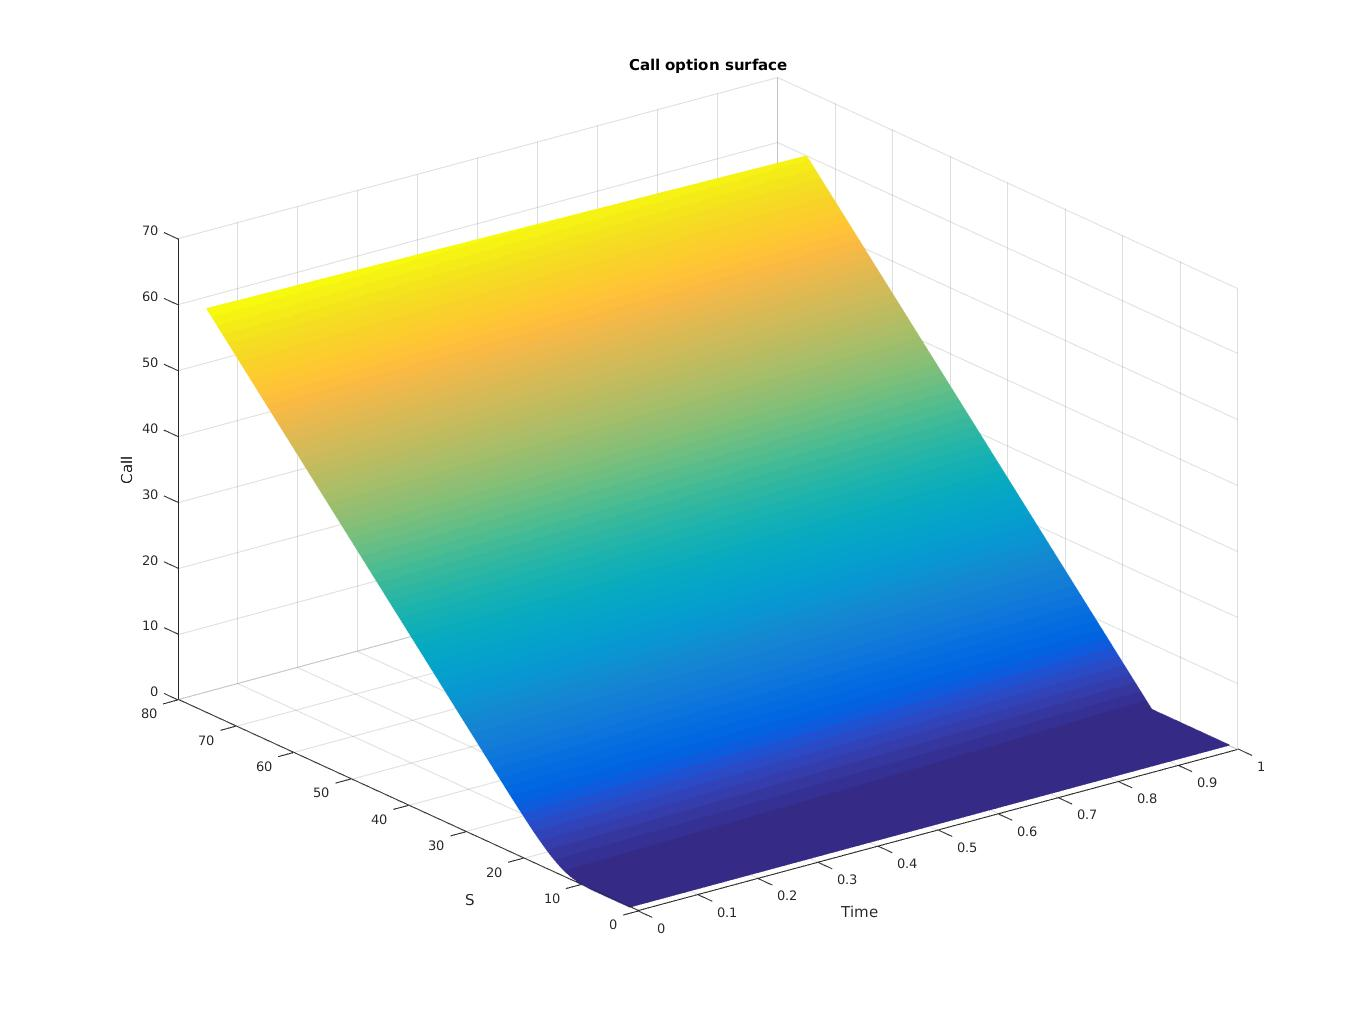
\includegraphics[width=0.8\linewidth]{BS_surface.jpg}
   \caption{Call option surface. It is computed with the parameters in table \ref{tab:BS}}
   \label{BS_surface} 
\end{figure}
$$
\left(
\begin{array}{c}
V^{n+1}_{1} \\
V^{n+1}_{2} \\
\vdots \\
V^{n+1}_{M-2} \\
V^{n+1}_{M-1} \\
\end{array}
\right) = 
\underbrace{
\left(
\begin{array}{ccccc}
b     & c  & 0 & \cdots  & 0 \\
a     & b  & c & 0  & 0  \\
0      & \ddots & \ddots &   \ddots     & 0  \\
\vdots & 0 & a & b  & c  \\
0      & 0 & 0 & a  & b \\
\end{array}
\right) }_{\mathcal{D}} \cdot
\left(
\begin{array}{c}
V^{n}_{1} \\
V^{n}_{2} \\
\vdots \\
V^{n}_{M-2} \\
V^{n}_{M-1} 
\end{array}
\right)
+ \underbrace{
\left(
\begin{array}{c}
 a V^{n}_{0} \\
  0 \\
 \vdots \\
 0 \\
c V^{n}_{M} \\
\end{array}
\right) }_{\mbox{B (boundary terms)}}
$$
The system 
$$ V^{n+1}_{i} = \mathcal{D} V^{n}_{i} + B \quad \mbox{ for } \quad 1 \leq i \leq M-1$$
can be solved easily for $V^{n}_{i}$ by inverting the matrix $\mathcal{D}$.
\begin{figure}[t]
   \centering
   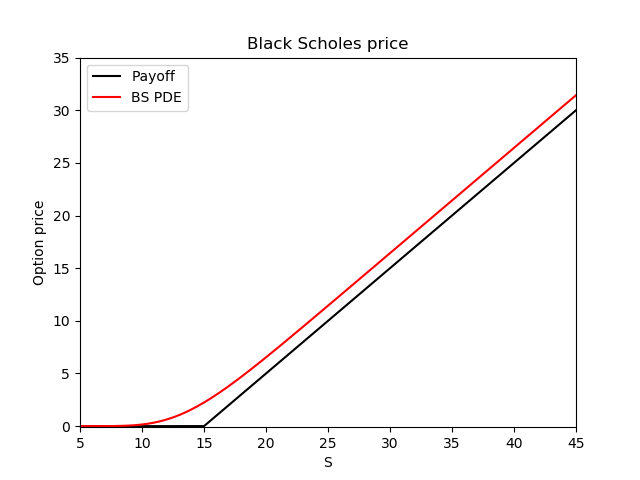
\includegraphics[width=0.7\linewidth]{BS_call.png}
   \caption{Price of a call option at time $t=0$ as a function of the underlying.}
   \label{BS_call}
\end{figure}  
\begin{table}[t]
\begin{center}
\begin{minipage}{0.8\linewidth}
\centering
 \begin{tabular}{||l|l|l|l||}
 \hline
  \multicolumn{4}{|c|}{Diffusion parameters} \\
  \hline
  $K$ & $T$ & $r$ & $\sigma$ \\
  \hline
  15 & 1 & 0.1 & 0.25 \\
  \hline
  \end{tabular}
  \caption{This table shows option's parameters and diffusion process parameters.}
  \label{tab:BS}
\end{minipage}
 \end{center}
\end{table}

Using the parameters in table (\ref{tab:BS}) we solve the fully implicit equation and plot the solution in Figures \ref{BS_surface} and \ref{BS_call}, as an example.



\subsection{Merton PIDE}

\begin{figure}[t]
   \centering
   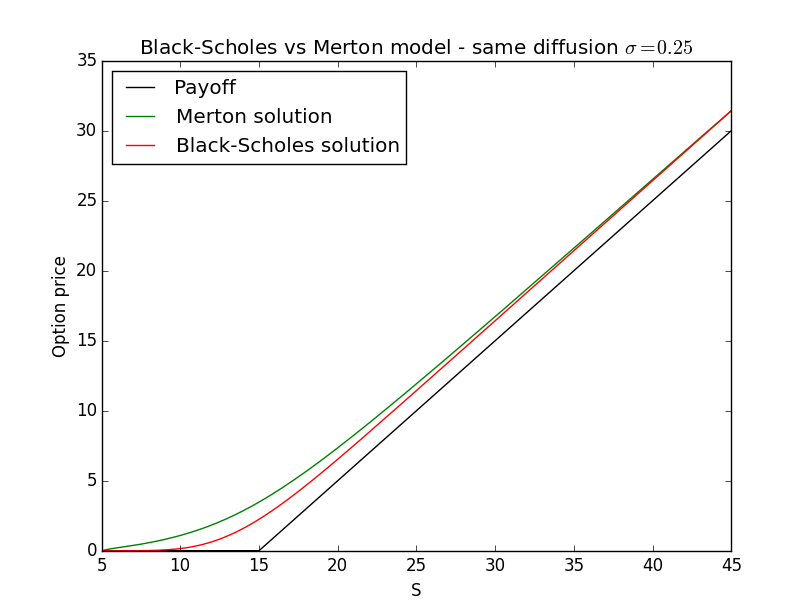
\includegraphics[width=0.7\linewidth]{BS_Merton.png}
   \caption{Comparison of prices of a call option at time $t=0$ for Merton and BS models. The used parameters are those in Tables \ref{tab:Mert} and \ref{tab:BS}}.
   \label{BS_Merton}
\end{figure}  
\begin{figure}[t]
   \centering
   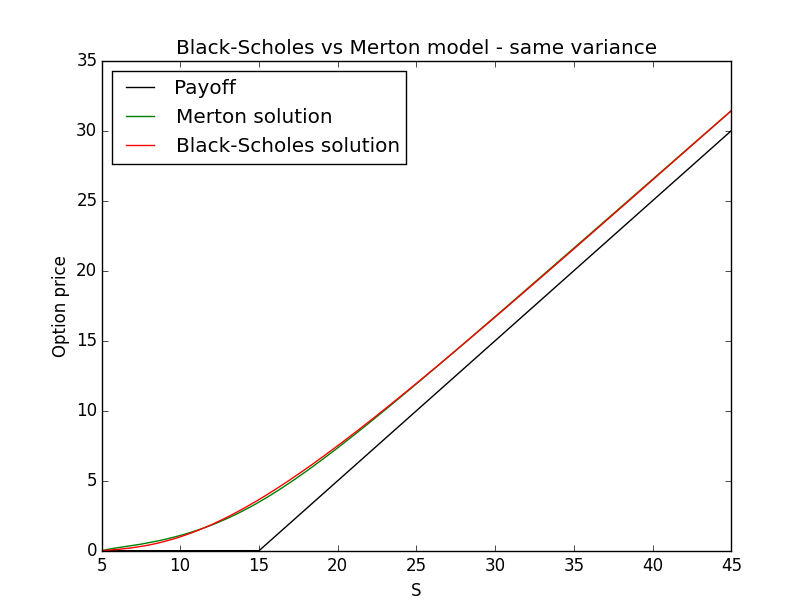
\includegraphics[width=0.7\linewidth]{BS_Merton2.png}
   \caption{Comparison of prices of a call option at time $t=0$ for Merton and BS models with same standard deviation $=0.25$.}
   \label{BS_Merton2} 
 \end{figure}
 \ \hspace{2mm} \hspace{3mm} \
 \begin{figure}[t]
  %\centering
   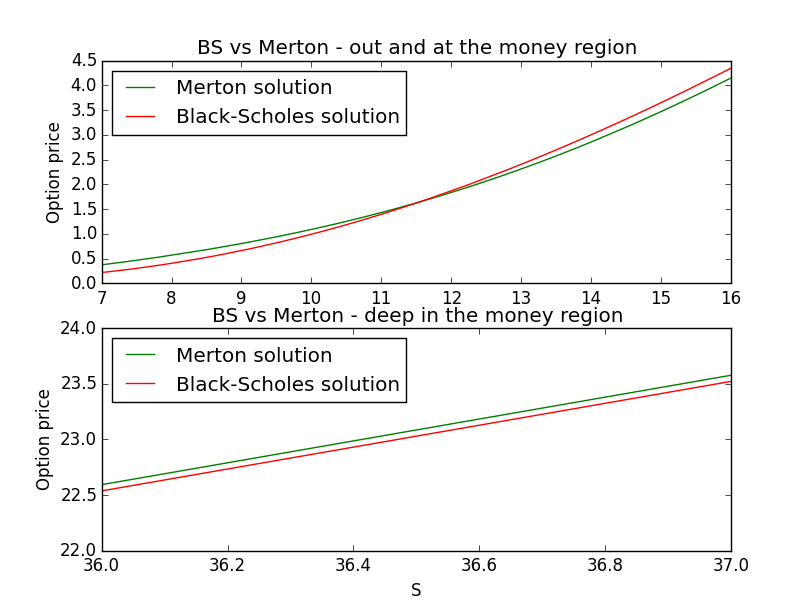
\includegraphics[width=0.7\linewidth]{BS_Merton3.png}
   \caption{Comparison of prices of a call option at time $t=0$ for Merton and BS models with same standard deviation $=0.25$. Zoom on the ITM and OTM regions.}
   \label{BS_Merton3}
\end{figure}
We presented the Merton model in the section (\ref{Merton_section}) and derived the Merton generator in Eq. (\ref{Merton_gen}). 
Recall that the jump component of the Merton process has finite activity, $\nu(\R) = \lambda < \infty$.
Following Eq. (\ref{PIDE_log}), the Merton PIDE in log-variables has the following form: 
\begin{align}\label{Merton_PIDE}
&  \frac{\partial V(t,x)}{\partial t} - r V(t,x) 
          + \biggl( r -\frac{1}{2}\sigma^2 -m \biggr) \frac{\partial V(t,x)}{\partial x} \\ \nonumber
          &+ \frac{1}{2} \sigma^2 \frac{\partial^2 V(t,x)}{\partial x^2} 
          + \int_{\R} V(t,x+z) \nu(dz) - \lambda V(t,x)  = 0.
\end{align}
with $m = \int_{\R} \bigl( e^z-1 \bigr) \nu(dz) = \lambda \bigl( e^{\alpha + \frac{1}{2} \xi^2} -1 \bigr)$. 
But since we have to restrict the unbounded domain to a bounded domain, we consider the equation (\ref{restricted_domain}):
\begin{align*}
&  \frac{\partial V(t,x)}{\partial t} - r V(t,x) 
          + \biggl( r -\frac{1}{2}\sigma^2 - \hat m \biggr) \frac{\partial V(t,x)}{\partial x} \\
          &+ \frac{1}{2} \sigma^2 \frac{\partial^2 V(t,x)}{\partial x^2} 
          + \int_{-B_1}^{B_2} V(t,x+z) \nu(dz) - \hat \lambda V(t,x)  = 0.
\end{align*}
with $\hat m = \int_{-B_1}^{B_2} \bigl( e^z-1 \bigr) \nu(dz)$ and $\hat \lambda = \int_{-B_1}^{B_2} \nu(dz)$.

In order to approximate the integral terms we use the trapezoidal quadrature rule with the same grid resolution, as in \cite{CoVo05b}. 
For $K_1,K_2 \in \R$ we choose $B_1,B_2$ such that $ \bigl[-B_1,B_2\bigr] = \bigl[ ( -K_1-1/2 )\Delta x , ( K_2+1/2 )\Delta x \bigr] $.
\begin{equation}\label{trap_quad}
 \int_{-B_1}^{B_2}  V(t_n,x_i+z) \nu(dz) \approx \sum_{k = -K_1}^{K_2} \nu_k V^{n}_{i+k}
\end{equation}
where
\begin{equation}\label{nu1}
 \nu_k = \int_{(k-\frac{1}{2}) \Delta x}^{(k+\frac{1}{2}) \Delta x} \nu(z) dz, \hspace{1em} \mbox{ for } \hspace{1em} -K_1 \leq k \leq K_2. 
\end{equation}
We can derive that $ \hat \lambda = \sum_{k = -K_1}^{K_2} \nu_k $. For large values of $B_1$ and $B_2$, the parameter $\hat \lambda$ is a good approximation for $\lambda$, since
$$\lambda = \lim_{B_1,B_2 \to \infty} \hat \lambda = \lim_{B_1,B_2 \to \infty} \int_{-B_1}^{B_2} \nu(dz).$$
The discretized equation using the IMEX scheme becomes: 
\begin{align}
&\frac{V^{n+1}_{i} -V^{n}_{i}}{\Delta t} + 
(r-\frac{1}{2}\sigma^2 - \hat m) \frac{V^{n}_{i+1} -V^{n}_{i-1}}{ 2 \Delta x} \\ \nonumber
&+ \frac{1}{2} \sigma^2 \frac{V^{n}_{i+1} + V^{n}_{i-1} - 2 V^{n}_{i}}{\Delta x^2}  - (r+\hat \lambda) V^{n}_i +\sum_{k = -K_1}^{K_2} \nu_k V^{n+1}_{i+k} = 0.
\end{align}
Rearranging the terms: 
\begin{align*}
\underbrace{ V^{n+1}_{i} + \Delta t \sum_{k = -K_1}^{K_2} \nu_k V^{n+1}_{i+k} }_{\tilde V^{n+1}_i} &= 
	V^{n}_{i} \biggl( 1 + (r+\hat \lambda)\Delta t + \sigma^2 \frac{\Delta t}{h_x^2} \biggr)  \\
& + V^{n}_{i+1} \biggl( -(r -\frac{1}{2}\sigma^2 -\hat m )\frac{\Delta t}{2 \Delta x} +
\frac{1}{2}\sigma^2 \frac{\Delta t}{\Delta x^2}  \biggr)  \\
& + V^{n}_{i-1} \biggl( (r -\frac{1}{2}\sigma^2 - \hat m)\frac{\Delta t}{2 \Delta x} + 
\frac{1}{2}\sigma^2 \frac{\Delta t}{\Delta x^2}  \biggr).
\end{align*}
We can rename the coefficients:
$$ \tilde V^{n+1}_{i} = a V^{n}_{i-1} + b V^{n}_{i} + c V^{n}_{i+1}, $$
and solve the system for $V^{n}_{i}$:
\begin{equation*}
 \begin{cases}
  \tilde V^{n+1}_i = V^{n+1}_{i} + \Delta t \sum_{k = -K_1}^{K_2} V^{n+1}_{i+k} \nu_k \\
  V^{n}_{i} = \mathcal{D}^{-1} \biggl( \tilde V^{n+1}_{i} - B \biggr) \quad \mbox{ for } \quad 1 \leq i \leq M-1  
 \end{cases}
\end{equation*}
by inverting the matrix $\mathcal{D}$, and with boundary terms $B = (a V^{n}_{0}, 0, ... , 0, c V^{n}_{M})$.  
\begin{table}[t]
 \begin{center}
 \begin{minipage}{0.8\linewidth}
  \centering
  \begin{tabular}{||l|l|l||l|l|l|l||}
  \hline
  \multicolumn{7}{|c|}{Merton parameters} \\
  \hline
  $K$ & $T$ & $r$ & $\sigma$ & $\alpha$ &$\xi$ & $\lambda$ \\
  \hline
  15 & 1 & 0.1 & 0.25 & 0 & 0.5 & 0.8 \\
  \hline
  \end{tabular}
  \caption{This table shows option's parameters and Merton process parameters.}
  \label{tab:Mert}
 \end{minipage}
 \end{center}
\end{table}
In Figure \ref{BS_Merton} we computed the prices using the parameters in tables \ref{tab:Mert} and \ref{tab:BS}. The Merton curve is higher than the BS curve. This is a consequence 
of the jump component that increases the total variance of the process. The two processes have same diffusion component $\sigma$, but in the Merton process the total variance is influenced
by the jumps as well, while in the BS the variance is just $\sigma^2$.

In order to compare the two models, we therefore compare two processes with the same variance. The Merton process has parameters as in Table \ref{tab:Mert}, while the BS process has a $\sigma$
such that it is equal to the standard deviation of the Merton process (see (\ref{Merton_moments}).
We show the comparison in figures \ref{BS_Merton2} and \ref{BS_Merton3}. We see that under the actual choice of parameters, there is not a very evident difference in the shape.
However, as expected the BS curve is higher than the Merton curve in the \emph{at the money} (ATM) region, and lower in the deep \emph{in the money} (ITM) 
and \emph{out of the money} (OTM) regions.
This is a consequence of the heavy tails distribution of the Merton process, that assigns more probability to the large movements of the underlying.  


\subsection{Variance Gamma PIDE}\label{VG_section2}

The last example we consider is the Variance Gamma process, already introduced in Section \ref{VG_section}. This is an infinite activity process
($\nu(\R) = \infty$). 
If we consider the exponential of the risk neutral process $(r-\omega)t + X_t$ where $X_t$ is a VG process with triplet as in Section \ref{VG_section}.
By the simple change of variable (\ref{log_var}) on the generator (\ref{VG_gen}), and adding the convection terms 
$(r-\omega) \frac{\partial V(t,x)}{\partial x}$, we can derive the VG PIDE for a function $V \in C^{1,1}(\R) \bigcap C_2(\R)$:
\begin{equation} \label{VG_PIDE}
 \frac{\partial V(t,x)}{\partial t} + (r-\omega) \frac{\partial V(t,x)}{\partial x}
 + \int_{\R \backslash \{0\}} \bigl[ V(t,x+z) - V(t,x) \bigr] \nu(dz) = rV(t,x) .
\end{equation}
But in this case, the previous method cannot be applied directly, because of the singularity in the integral.

The idea for general infinite activity processes is to come down to a non-singular case by approximating the process $X_t$ by an
appropriate finite activity process with a modified diffusion component.
We can approximate the ``small jumps'' martingale component with a Brownian motion with the same variance.
After fixing a truncation parameter $\epsilon >0$, we can split the integrals in the SDE into two domains: $\{|z|<\epsilon\}$ and $\{|z|\geq \epsilon\}$.
The integrand on the domain $\{ |z|<\epsilon \}$, is approximated by the Taylor expansion 
 $e^z-1-z = \frac{z^2}{2} + \mathcal{O}(z^3)$ such that
\begin{align}\label{log_sde_inf_act}\nonumber
  dX_t =& \biggl( \mu-\frac{1}{2}\sigma^2 - \int_{\R} \bigl( e^z-1-z \bigr) \nu(dz) \biggr)dt + \sigma dW + + \int_{\R} z \tilde N(dt,dz) \\ \nonumber
       =& \biggl( \mu - \frac{1}{2}\sigma^2 -\int_{|z|<\epsilon} (e^z-1-z) \nu(dz) -\int_{|z|\geq \epsilon} (e^z-1-z) \nu(dz)  \biggr) dt\\ \nonumber
        &+ \sigma dW_t + \underbrace{\int_{|z|< \epsilon} z \tilde N(dt,dz)}_{\sigma_{\epsilon} dW_t} + \int_{|z| \geq \epsilon} z \tilde N(dt,dz) \\ 
       =& \biggl( \mu - \frac{1}{2} (\sigma^2 + \sigma_{\epsilon}^2) - \omega_{\epsilon} + \lambda_{\epsilon} \theta_{\epsilon}  \biggr) dt + \bigl( \sigma+\sigma_{\epsilon}\bigr) dW_t 
       + \int_{|z|\geq \epsilon} z \tilde N(dt,dz) ,
\end{align}
where we defined the new parameters
\begin{align}\label{sig_eps}
 & \sigma_{\epsilon}^2 =  \int_{|z| < \epsilon} z^2 \nu(dz), \quad \quad \omega_{\epsilon} = \int_{|z| \geq \epsilon} (e^z-1) \nu(dz), \\ \nonumber
 & \lambda_{\epsilon} =  \int_{|z| \geq \epsilon} \nu(dz), \quad \quad \theta_{\epsilon} = \frac{1}{\lambda_{\epsilon}} \int_{|z| \geq \epsilon} z \nu(dz) .
\end{align}
The process $\int_{|z|\geq \epsilon} z \tilde N(dt,dz)$ is a compensated Poisson process with finite activity $\lambda_{\epsilon}$ 
and variance $\sigma_J^2 = \int_{|z| \geq \epsilon} z^2 \nu(dz) $.

In the case of the VG process, where $\sigma = 0$ we have the following dynamics for $X_t$
\begin{equation}\label{log_sde_VG}
dX_t = \biggl( \mu - \frac{1}{2} \sigma_{\epsilon}^2 - \omega_{\epsilon} + \lambda_{\epsilon} \theta_{\epsilon}  \biggr) dt 
       + \sigma_{\epsilon} dW_t + \int_{|z|\geq \epsilon} z \tilde N(dt,dz)
\end{equation}
For any $V\in C^2(\R) \bigcap C_2(\R)$, the associated infinitesimal generator has a jump-diffusion form
\begin{align}\label{VG_inf_gen}
\LL^{VG} V(x) \; =& \; \bigl( \mu-\frac{1}{2}\sigma_{\epsilon}^2 - w_{\epsilon} \bigr) \frac{\partial V}{\partial x} 
+ \frac{1}{2}\sigma_{\epsilon}^2 \frac{\partial^2 V}{\partial x^2} \\ \nonumber
&+ \int_{|z| \geq \epsilon} V(x+z) \nu(dz) - \lambda_{\epsilon} V(x).
\end{align}
\begin{figure}[t]
   \centering
   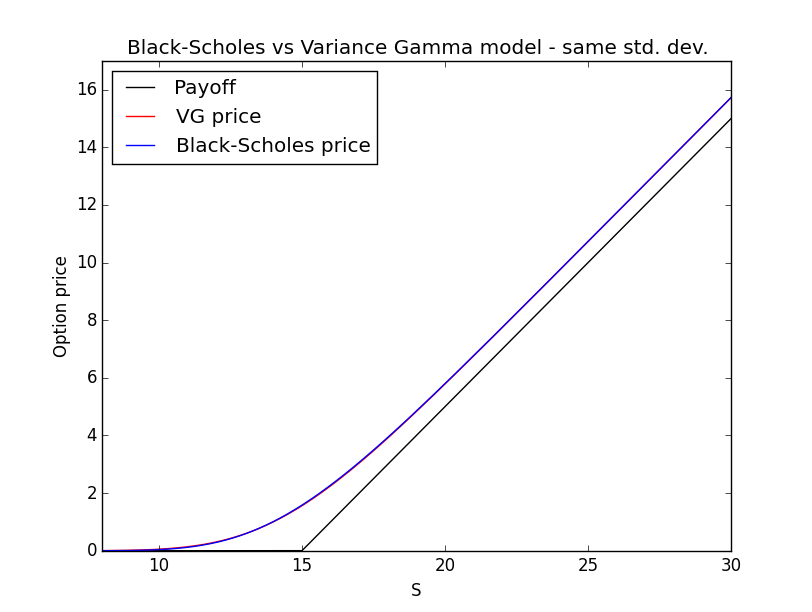
\includegraphics[width=0.7\linewidth]{BS_VG.png}
   \caption{Comparison of prices of a call option at time $t=0$ for VG and BS models with same standard deviation.}
   \label{BS_VG} 
 \end{figure}
 \begin{figure}[t]
  %\centering
   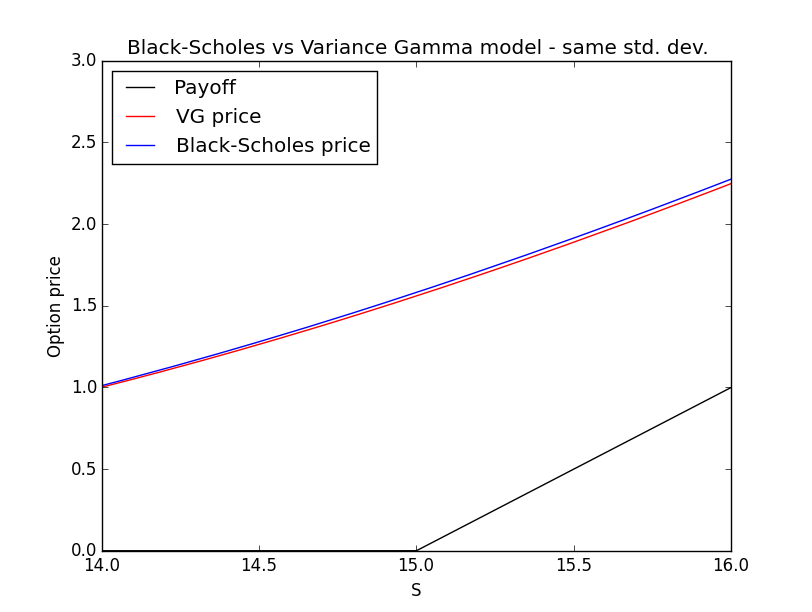
\includegraphics[width=0.7\linewidth]{BS_VG_ATM.png}
   \caption{Comparison of prices of a call option at time $t=0$ for VG and BS models with same standard deviation. Zoom on the ATM region.}
   \label{BS_VG_ATM}
\end{figure}
The same result can be obtained directly from the infinitesimal generator (\ref{RN_log_gen}) with $\sigma =0$:
\begin{align*}
\LL^{VG} V(x) =& \; \mu \frac{\partial V}{\partial x}
+ \int_{|z| < \epsilon}
\biggl[ V(x+z) - V(x) - (e^z-1)\frac{\partial V}{\partial x} \biggr] \nu(dz) \\
&+ \int_{|z| \geq \epsilon}
\biggl[ V(x+z) - V(x) - (e^z-1)\frac{\partial V}{\partial x} \biggr] \nu(dz),
\end{align*}
In the integral term on the domain $\{ |z|<\epsilon \}$, we use the Taylor approximation
\begin{itemize}
 \item $V(x+z) = V(x) + \frac{\partial V}{\partial x} z + \frac{1}{2} \frac{\partial^2 V}{\partial x^2} z^2 + \mathcal{O}(z^3)$.
 \item $e^z-1 = z + \frac{z^2}{2} + \mathcal{O}(z^3) $.
\end{itemize}
Considering only the terms up to the second order, the integral for $\{ |z| < \epsilon \}$ is
\begin{equation*}
 \int_{|z| < \epsilon} \frac{z^2}{2}
\biggl[ \frac{\partial^2 V}{\partial x^2} - \frac{\partial V}{\partial x} \biggr] \nu(dz)
= \frac{\sigma_{\epsilon}^2}{2} \biggl[ \frac{\partial^2 V}{\partial x^2} - \frac{\partial V}{\partial x} \biggr],
\end{equation*}
and we get again the infinitesimal generator (\ref{VG_inf_gen}).
Using this generator and equations (\ref{derivative_PIDE}) and (\ref{mu=r}), the final PIDE is thus
\begin{align}\label{VG_JD}
&  \frac{\partial V(t,x)}{\partial t} +
 \bigl( r-\frac{1}{2}\sigma_{\epsilon}^2 - w_{\epsilon} \bigr) \frac{\partial V(t,x)}{\partial x} 
 + \frac{1}{2}\sigma_{\epsilon}^2 \frac{\partial^2 V(t,x)}{\partial x^2} \\ \nonumber
 &+ \int_{|z| \geq \epsilon} V(t,x+z) \nu(dz) = (\lambda_{\epsilon} + r) V(t,x).
\end{align}
This equation is very similar to equation (\ref{Merton_PIDE}), except for the truncation in the integral. 
At this point we can restrict the computational domain on $]-A_1,A_2[$ and the integral region on $[-B_1,B_2]$ and using the same discretization
used for the Merton PIDE, we can solve the problem by an IMEX scheme.\\
The IMEX scheme is monotone, stable and consistent (see (\cite{CoVo05b})).
\begin{table}[h!]
\begin{center}
 \begin{minipage}{0.8\linewidth}
  \centering
 \begin{tabular}{||l|l|l|l||l|l||}
\hline
  \multicolumn{6}{|c|}{VG parameters} \\
 \hline
$K$ & $T$ & $r$ & $\theta$ & $\sigma$ &$\kappa$  \\
\hline
15 & 1 & 0.1 & -0.1 & 0.2 & 0.1 \\
\hline
\end{tabular}
  \caption{This table shows option's parameters and VG process parameters.}
  \label{tab:VG}
\end{minipage}
  \end{center}
\end{table}
Using the parameters in Table \ref{tab:VG} we compute the call option prices for the VG process and compare them with the prices of a BS process with the same variance.
In figures \ref{BS_VG} and \ref{BS_VG_ATM} we show the comparison between the two curves, but under this choice of parameters, the difference in the shapes is not very relevant.
A zoom in the ATM region shows that the BS price is slightly higher than the VG price. The reason, analogue to what we saw in figure \ref{BS_Merton3}, is that the VG distribution
gives more mass to the tails and less to the center.

The reader can consult \cite{Schoutens} for further numerical tests on the calibration of exponential Lévy processes, such as Merton and VG processes. 



